\documentclass[12pt]{article}
\usepackage[a4paper, margin=1in]{geometry}
\usepackage{amsmath, amssymb, amsthm}
\usepackage{graphicx}
\graphicspath{{figures/}}
\usepackage{booktabs}
\usepackage{setspace}
\usepackage{hyperref}
\usepackage{caption}
\usepackage{float}
\usepackage{multirow}
\usepackage{color}
\usepackage{titling}
\usepackage{authblk}
\usepackage{xcolor}
\usepackage{tikz}
\usetikzlibrary{arrows.meta, positioning, decorations.pathreplacing}
\usepackage[T1]{fontenc}
\usepackage{lmodern}   % scalable Computer Modern
\usepackage{fix-cm}    % allow arbitrary sizes with \fontsize

% Title sizing
\title{\fontsize{22pt}{26pt}\selectfont
School absence works, sick leave is uncertain: an age-structured, channel-resolved evaluation of influenza absenteeism policies in Korea}

% Fonts for authors/affils
\renewcommand\Authfont{\fontsize{14pt}{18pt}\selectfont}
\renewcommand\Affilfont{\small\itshape}
\makeatletter
% Adjust spacing between affiliations
\renewcommand\AB@affilsepx{\\[0.25ex]}
% Remove ONLY the auto numeric author notes (the extra "1")
\renewcommand\AB@authnote[1]{}%
% Remove the automatic "and" before the last author
\renewcommand\Authsep{, }
\renewcommand\Authands{, }
\makeatother

% Authors (manual superscripts)
\author{Hyunwoo Cho\textsuperscript{}}
% Affiliations
\affil[]{}
\date{}

% Define theorem environments
\theoremstyle{plain}
\newtheorem{theorem}{Theorem}[section] % Numbered within sections
\newtheorem{lemma}[theorem]{Lemma}     % Lemmas share the numbering with theorems
\newtheorem{corollary}[theorem]{Corollary}
\newtheorem{remark}[theorem]{Remark}
\theoremstyle{remark}
\theoremstyle{definition}
\newtheorem{definition}[theorem]{Definition}

\begin{document}
\maketitle

\begin{abstract}
\noindent\textbf{Background.} Absenteeism-based interventions --- keeping infectious workers home (sick leave) or infectious children out of school --- are widely assumed to reduce influenza transmission, and are usually evaluated by the \emph{magnitude} of infection they avert. For an age-structured pathogen this framing omits three things: transmission removed from one channel (workplace or school) is not eliminated but \emph{redistributed} to others, particularly the household; a substantial fraction of onward transmission is \emph{presymptomatic} and therefore escapes any symptom-triggered absenteeism; and the effect can differ across age groups and across the timing of the intervention relative to the school calendar. Whether a given policy helps, and whom it helps, is therefore an empirical question that a single effect-size number cannot answer.

\noindent\textbf{Methods.} We built an age-structured deterministic SVEIR model for the Seoul Capital Area with 15 age groups, an Erlang-distributed infectious period ($I_1 I_2 I_3$) that separates a presymptomatic stage ($I_1$) from the symptomatic stages ($I_2, I_3$), and four contact channels (home, work, school, other), calibrated to National Health Insurance Service (NHIS) claims data across three normal seasons (2016--17, 2017--18, 2019--20). School-calendar changes in contact frequency were captured by a time-switching contact matrix; intervention intensity by a within-home crowding term acting on symptomatic absentees; and presymptomatic transmission by a stage-specific infectiousness weight. Channel allocation and season-specific reproduction numbers were estimated by a three-season joint No-U-Turn Sampler (NUTS) run (4000 post-warmup draws, zero divergences), and sick-leave and school-absence policies were compared at matched intensity by posterior forward simulation with credible intervals.

\noindent\textbf{Results.} First, \emph{school absence is confidently effective}: averted infection was $+1.6$ to $+3.4\%$ and every age band in every season showed a credible reduction (all $0 \notin$ CI). By contrast \emph{sick leave's net benefit is small and uncertain}: averted infection was $+0.2$ to $+0.5\%$ and its credible interval included zero in two of three seasons. Second, school absence averted far more infection than sick leave --- roughly fivefold in absolute counts (2019--20: 123{,}147 vs 23{,}492 infections averted) --- because the school channel, small in transmission share ($\pi_{\mathrm{school}} \approx 0.065$) but child-dominated, is the epidemic's engine; this ordering held under the credible intervals. Third, sick leave \emph{redistributes} rather than simply reduces: adult infection fell while school-age children's rose, a direction reproduced in all three independently fitted seasons, but the magnitude was small and statistically significant only in part (so we characterise it as a redistribution tendency, not established harm to children). The direction differed by metric --- channel-adjacent age groups in attack-rate terms, adults in absolute counts. Fourth, the redistribution toward children was larger during school vacation than during term, because sick-leave spillover flows through the always-open home channel; the direction was consistent but its magnitude was sensitive to immunity and crowding assumptions, so we describe it as redistribution that \emph{intensifies during vacation} rather than a clean sign reversal. The joint calibration also identified the workplace transmission share, $\pi_{\mathrm{work}} = 0.298$ (95\% CI $[0.241, 0.356]$), which single-season fits cannot resolve.

\noindent\textbf{Conclusions.} For an age-structured pathogen with presymptomatic transmission, school-based measures are both more effective and more certain than sick leave, and are free of the household-spillover hazard. Sick leave's population-level benefit is small and not robustly established; where used, it should be paired with household-isolation support, especially during winter holidays when its redistribution toward children is largest. Policy appraisal should be reframed from a single effect size to ``who bears the risk, and when.''
\end{abstract}

\noindent\textbf{Keywords:} seasonal influenza; age-structured transmission; sick leave; school absenteeism; household spillover; presymptomatic transmission; non-pharmaceutical interventions

\section{Introduction}
Keeping infectious individuals out of a shared setting --- paid sick leave for symptomatic workers, and school exclusion for symptomatic children --- is a standard non-pharmaceutical response to seasonal and pandemic influenza. The intuitive case is that an infectious person who stays home cannot infect the colleagues or classmates they would otherwise have met, so removing them lowers total infection. Evaluations have accordingly concentrated on the \emph{size} of that reduction.

For an age-structured respiratory pathogen this framing omits four things. First, the population is not homogeneous: susceptibility, clinical attack rate, and contact patterns vary sharply by age, and children are both among the most susceptible and, in most seasons, the most infectious group \cite{Jayasundara2014,Cauchemez2009}. A case prevented among adults is not equivalent to a case prevented among children. Second, sending an infectious person home does not end their transmission; it \emph{relocates} it into the household, whose age composition differs entirely from the setting they left. An infectious adult kept from work exposes, above all, their own children. Third, symptom-triggered absenteeism cannot act on transmission that occurs before symptoms: a meaningful share of influenza~A transmission is \emph{presymptomatic} \cite{NatureHealth2026,Lau2010}, and that share escapes any policy keyed to staying home when sick. Fourth --- and least appreciated --- \emph{when} the policy is applied matters, because the household is always open even when schools are not. A measure that merely shifts transmission into the home behaves differently during term time, when children are dispersed at school, than during a holiday, when they are at home all day.

These features interact in ways an effect-size analysis cannot see. Sick leave takes an infectious adult out of an adult-dominated setting and relocates their residual, post-symptomatic transmission into the household, toward children; school absence takes an infectious child out of a child-dominated setting and relocates transmission toward co-resident adults. The two levers are not two instances of one ``reduce contact'' mechanism but act on different channels and different ages. And because the sick-leave pathway runs through the home rather than the school, its burden on children depends on how much time children spend at home --- which the school calendar governs.

We argue that the outcome of an absenteeism policy is determined by dimensions the effect-size literature collapses: the \emph{direction} in which it redistributes transmission along the age gradient of vulnerability, the \emph{metric} used to read that redistribution, and the \emph{timing} of the intervention relative to the epidemic and the school calendar. This reframes the evaluation question from ``how much does the policy avert'' to ``whom does it move the risk toward, with what certainty, and when.''

To examine this we developed an age-structured metapopulation SVEIR model of seasonal influenza in the Seoul Capital Area, with an Erlang-distributed infectious period that isolates a presymptomatic stage, four explicitly separated contact channels, and a physically grounded representation of what absenteeism does to contacts, calibrated to three normal seasons of NHIS claims data and equipped with full posterior credible intervals from a three-season joint NUTS calibration. The model lets us (i) compare sick-leave and school-absence policies at matched intensity on the same footing and with credible intervals; (ii) locate where in the workplace-transmission / crowding parameter space sick leave helps versus harms; (iii) decompose outcomes by age and by metric; and (iv) ask how the same sick-leave policy behaves in different phases of the epidemic, split naturally by the winter-vacation calendar.

We report four findings. School absence is confidently effective across all seasons and age groups, whereas sick leave's net benefit is small and, in two of three seasons, not distinguishable from zero. School absence averts far more infection than sick leave --- roughly fivefold in counts --- because the school channel drives the epidemic despite its small fitted transmission share. Sick leave redistributes rather than reduces, moving infection from adults toward school-age children in direction across all three seasons, though with a magnitude small enough that the redistribution is only partly significant and should be read as a tendency rather than established harm. And that redistribution toward children is larger during school vacation than during term, because its spillover flows through the always-open home channel. The unifying message is that absenteeism policy for age-structured pathogens should be judged by who bears the redistributed risk, with what certainty, and when the policy is applied --- not by an aggregate effect size.

\section{Model Description}
\label{sec:model}
This section defines the model structure --- compartments, flows, force of infection, and the mechanisms for presymptomatic transmission, household spillover, the school calendar, and vaccination --- in symbolic form. Numerical values of every parameter are collected in Section~\ref{sec:parameters}, and the procedures used to calibrate and exercise the model in Section~\ref{sec:methods}.

\subsection{Compartmental structure and flow}
We model seasonal influenza in the Seoul Capital Area as an age-structured SVEIR (susceptible--vaccinated--exposed--infectious--recovered) system stratified into 15 five-year age groups ($0$--$4$, $5$--$9$, \dots, $65$--$69$, $70+$). For each age group $a$, susceptibles $S_a$ acquire vaccine-derived leaky protection (moving to $V_a$, efficacy $\mathrm{VE}$) at the time-dependent vaccination hazard $v(t)$, or become exposed $E_a$ at the force of infection $\lambda_a(t)$; vaccinated individuals may still be infected, at reduced hazard $(1-\mathrm{VE})\lambda_a$. Exposed individuals become infectious at rate $\sigma$. The infectious period is Erlang-distributed with three sub-stages $I_{1,a} \to I_{2,a} \to I_{3,a}$, each left at rate $3\gamma$ (so the mean infectious period is $1/\gamma$); the shape follows Wearing et al.\ \cite{Wearing2005} and, crucially here, gives the model a distinct \emph{presymptomatic} sub-stage $I_1$ (Section~\ref{sec:presymp}). The flow is shown in Figure~\ref{fig:flow}, and the governing equations for each age group $a$ are
\begin{align}
\frac{dS_a}{dt}   &= -\lambda_a S_a - v(t)\,S_a, &
\frac{dV_a}{dt}   &= v(t)\,S_a - (1-\mathrm{VE})\,\lambda_a V_a, \notag\\
\frac{dE_a}{dt}   &= \lambda_a S_a + (1-\mathrm{VE})\,\lambda_a V_a - \sigma E_a, &
\frac{dI_{1,a}}{dt}&= \sigma E_a - 3\gamma\, I_{1,a}, \\
\frac{dI_{2,a}}{dt}&= 3\gamma\, I_{1,a} - 3\gamma\, I_{2,a}, &
\frac{dI_{3,a}}{dt}&= 3\gamma\, I_{2,a} - 3\gamma\, I_{3,a}, \notag\\
\frac{dR_a}{dt}   &= 3\gamma\, I_{3,a}. \notag
\end{align}

\begin{figure}[H]
\centering
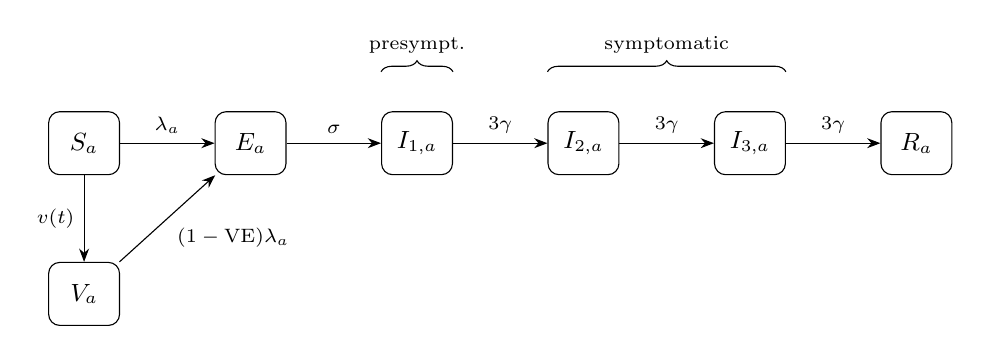
\begin{tikzpicture}[
  >=Stealth, node distance=11mm and 12mm,
  box/.style={draw, rounded corners, minimum width=9mm, minimum height=8mm, font=\small},
  lab/.style={font=\scriptsize}
]
\node[box] (S) {$S_a$};
\node[box, below=of S] (V) {$V_a$};
\node[box, right=of S] (E) {$E_a$};
\node[box, right=of E] (I1) {$I_{1,a}$};
\node[box, right=of I1] (I2) {$I_{2,a}$};
\node[box, right=of I2] (I3) {$I_{3,a}$};
\node[box, right=of I3] (R) {$R_a$};
\draw[->] (S) -- node[above,lab]{$\lambda_a$} (E);
\draw[->] (S) -- node[left,lab]{$v(t)$} (V);
\draw[->] (V) -- node[below right,lab]{$(1-\mathrm{VE})\lambda_a$} (E);
\draw[->] (E) -- node[above,lab]{$\sigma$} (I1);
\draw[->] (I1) -- node[above,lab]{$3\gamma$} (I2);
\draw[->] (I2) -- node[above,lab]{$3\gamma$} (I3);
\draw[->] (I3) -- node[above,lab]{$3\gamma$} (R);
\draw[decorate, decoration={brace, amplitude=4pt}] ([yshift=5mm]I1.north west) -- ([yshift=5mm]I1.north east)
  node[midway, above=3pt, lab]{presympt.};
\draw[decorate, decoration={brace, amplitude=4pt}] ([yshift=5mm]I2.north west) -- ([yshift=5mm]I3.north east)
  node[midway, above=3pt, lab]{symptomatic};
\end{tikzpicture}
\caption{Compartmental flow for each age group $a$. The infectious period is an Erlang(3) chain; $I_1$ is presymptomatic (infectious at reduced weight $w$, not subject to absenteeism), $I_2$ and $I_3$ are symptomatic (subject to policy). Symptom onset, and the observation model, are placed at the $I_1 \to I_2$ transition.}
\label{fig:flow}
\end{figure}

\subsection{Force of infection and contact channels}
\label{sec:foi}
The force of infection is separated into four contact channels $c \in \{\mathrm{home},\mathrm{work},\mathrm{school},\mathrm{other}\}$. Writing $I_{1,b}$ and $I_{23,b} = I_{2,b} + I_{3,b}$ for the presymptomatic and symptomatic prevalences in age group $b$, the channel hazards are
\begin{align}
\lambda^{\mathrm{work}}_a   &= \phi_a\, s_f(t)\, \beta_{\mathrm{work}} \sum_b C^{\mathrm{work}}_{ab}(t)\, \frac{w\,I_{1,b} + p_{\mathrm{work}}\, I_{23,b}}{N_b}, \\
\lambda^{\mathrm{school}}_a &= \phi_a\, s_f(t)\, \beta_{\mathrm{school}} \sum_b C^{\mathrm{school}}_{ab}(t)\, \frac{w\,I_{1,b} + p_{\mathrm{school}}\, I_{23,b}}{N_b}, \\
\lambda^{\mathrm{home}}_a   &= \phi_a\, s_f(t)\, \beta_{\mathrm{home}} \sum_b C^{\mathrm{home}}_{ab}(t)\, \frac{w\,I_{1,b} + \bigl(1 + \kappa_b (1-p)_b\bigr) I_{23,b}}{N_b}, \\
\lambda^{\mathrm{other}}_a  &= \phi_a\, s_f(t)\, \beta_{\mathrm{other}} \sum_b C^{\mathrm{other}}_{ab}(t)\, \frac{w\,I_{1,b} + I_{23,b}}{N_b}.
\end{align}
with total hazard $\lambda_a(t) = \sum_c \lambda^c_a(t)$. Here $\phi_a$ is age-specific relative susceptibility, $s_f(t)$ a seasonal forcing term, $\beta_c$ the transmissibility weight of channel $c$, and $C^{c}_{ab}(t)$ the time-dependent contact matrix of channel $c$ between age groups $a$ and $b$ (age-structured contact matrices follow the POLYMOD approach \cite{Mossong2008}). The presymptomatic block $w\,I_1$ passes through unaffected in every channel; the policy retention fractions $p_{\mathrm{work}}, p_{\mathrm{school}}$ (Section~\ref{sec:spillover}) and the home crowding term $\kappa_b (1-p)_b$ act only on the symptomatic block $I_{23}$.

\subsection{Presymptomatic transmission and the observation model}
\label{sec:presymp}
The first infectious sub-stage $I_1$ represents the presymptomatic phase: individuals are infectious but not yet symptomatic. Symptoms --- and hence any symptom-triggered behaviour (care-seeking, absenteeism) --- begin at the $I_1 \to I_2$ transition, so we place the \emph{observation} model (NHIS claims) at symptom onset and let both policies act only on the symptomatic stages $I_2, I_3$. Presymptomatic individuals transmit at a reduced relative infectiousness $w$; every channel's force of infection therefore weights $I_1$ by $w$ and $I_2 + I_3$ by unity. The value of $w$ (Section~\ref{sec:parameters}) follows a recent household study of influenza~A \cite{NatureHealth2026} and earlier shedding estimates \cite{Lau2010}; influenza~B shows no clear evidence of presymptomatic transmission, so applying an A-based weight throughout is a conservative choice.

Because absenteeism cannot touch presymptomatic transmission, the presymptomatic stage sets a ceiling on what any symptom-based policy can achieve. This mechanism is what makes sick leave's effect on total infection modest: much of the transmission a sick worker would generate has already occurred, or occurs through $I_1$ contacts the policy does not reach.

\subsection{Household spillover under absenteeism}
\label{sec:spillover}
Absenteeism is represented as additional within-home transmission incurred when symptomatic individuals who would otherwise have attended work or school instead remain at home. Baseline attendance is described by a retention fraction $p$ (the fraction who keep attending while symptomatic), so $1-p$ is the fraction sent home; the policy raises the intervention intensity by lowering $p$ (Section~\ref{sec:policy}). Only the symptomatic block $I_{23}$ is affected --- presymptomatic individuals are, by definition, not yet identifiable as sick --- and the home-channel symptomatic prevalence is scaled by
\begin{equation}
1 + \kappa_b\,(1-p)_b ,
\end{equation}
where $\kappa_b$ is the per-group increase in effective household transmission from a symptomatic individual spending the day at home, and $(1-p)_b$ is the group-specific sent-home fraction:
\begin{equation}
(1-p)_b =
\begin{cases}
1 - p_{\mathrm{school}}, & \text{students},\\
\rho_b\,(1 - p_{\mathrm{work}}), & \text{workers},\\
0, & 70+,
\end{cases}
\end{equation}
with $\rho_b$ the measured employment rate (students take $\rho_b = 0$, i.e.\ no commute). We deliberately write the spillover through $1-p$ rather than introducing a separate ``retained-fraction'' symbol: the retention $p$ already carries this information, and the crowding coefficient $\kappa$ is the only genuinely new quantity. The crowding coefficients are derived independently --- not fitted --- from a national time-use survey, and their construction and values are given in Section~\ref{sec:par_kappa}.

\subsection{Time-switching contact matrix \texorpdfstring{$C(t)$}{C(t)}}
\label{sec:ctime}
The school calendar enters the model through the contact matrix, not the transmissibility coefficient. Each channel's matrix is a trapezoidal-in-time blend of an empirically measured term-time matrix and vacation matrix,
\begin{equation}
C^{c}_{ab}(t) = \bigl(1 - h(t)\bigr)\, C^{c,\mathrm{term}}_{ab} + h(t)\, C^{c,\mathrm{vacation}}_{ab},
\end{equation}
where $C^{\mathrm{term}}$ and $C^{\mathrm{vacation}}$ are separate NIMS contact surveys measured during term and during vacation \cite{NIMS} --- consistent with the marked holiday reduction in school-age contacts reported elsewhere \cite{Eames2012} and in Korean contact surveys \cite{Son2025} --- and $h(t)$ is the winter-vacation calendar (a trapezoidal ramp; dates in Section~\ref{sec:parameters}); all four channels switch together. This matters because an earlier version encoded vacation as a multiplier on $\beta_{\mathrm{school}}$, which conflates contact \emph{number} with transmissibility \emph{per contact} and spuriously inflated the baseline home force of infection during vacation. Moving the calendar into $C(t)$ makes the baseline spillover factor identically $1.0$ across the year (verified numerically), so that contact \emph{frequency} is handled by $C(t)$ and intervention \emph{intensity} by $\kappa$, and the two never contaminate each other.

\subsection{Vaccination}
\label{sec:vax}
Vaccine uptake enters as a time-distributed hazard normalized to reach a target coverage $C$ over the finite season,
\begin{equation}
v(t) = \frac{-\ln(1 - C)}{Z}\, \mathrm{density}(t),
\end{equation}
where $-\ln(1 - C)$ converts target coverage to cumulative hazard, $\mathrm{density}(t)$ is the seasonal uptake shape, and $Z$ normalizes it over $[0,365]$. This hazard transform reproduces the target vaccinated fraction essentially exactly, correcting an earlier density-scaling implementation that undershot coverage.

\subsection{Transmissibility allocation}
\label{sec:reparam}
To separate the scale of transmission from its allocation across channels, we write
\begin{equation}
\beta_c = \frac{R_0}{\rho_{\mathrm{eff}}(\pi,\phi)}\,\pi_c,
\qquad \textstyle\sum_c \pi_c = 1,
\end{equation}
where $R_0$ sets the size (data-determined) and $\pi = (\pi_{\mathrm{home}}, \pi_{\mathrm{work}}, \pi_{\mathrm{school}}, \pi_{\mathrm{other}})$ sets the allocation. Here $\rho_{\mathrm{eff}}$ is the dominant eigenvalue of the next-generation operator, adjusted for presymptomatic infectiousness: because $I_1$ transmits at reduced weight $w$, the effective spectral scaling is $\rho_{\mathrm{eff}} = \rho\cdot(w+2)/3$, and using $\rho_{\mathrm{eff}}$ keeps $\beta$ and $R_0$ mutually consistent. The allocation $\pi$ is informed by channel-specific priors and, decisively, by multi-season data (Section~\ref{sec:methods}); prior strengths are listed in Section~\ref{sec:par_pins}.

\section{Parameters}
\label{sec:parameters}
This section collects the numerical values of every model parameter, verified directly against the calibrated implementation. Fixed epidemiological constants are in Table~\ref{tab:param_epi}; the age-specific vectors ($\phi_a$, reporting fraction, initial immunity, crowding, employment) in Table~\ref{tab:param_age}; contact structure and spatial scope in Table~\ref{tab:param_contact}; policy parameters in Table~\ref{tab:param_policy}; seasonality and vaccination in Table~\ref{tab:param_seasonality}; Bayesian priors and posteriors in Tables~\ref{tab:param_bayes}--\ref{tab:param_pins}; and initial conditions and solver settings in Tables~\ref{tab:param_init}--\ref{tab:param_solver}. The subsections below explain the parameters that require justification.

\subsection{Age-specific susceptibility \texorpdfstring{$\phi$}{phi}}
Relative susceptibility $\phi_a$ follows a linear U-shape, anchored to the literature at three points --- a child value of $2.0$ \cite{Cauchemez2009,Layan2024}, a working-age floor of $1.0$, and an elderly value of $1.5$ \cite{Panatto2018} --- with intermediate bands interpolated linearly, consistent with age-specific attack-rate evidence \cite{Jayasundara2014}.

\subsection{Reporting fractions \texorpdfstring{$\gamma_{\mathrm{report}}$}{gamma\_report}}
Age-specific claims/reporting fractions follow CDC-style estimates \cite{Reed2015}, with the adolescent ($15$--$19$) band assigned an adult-level value rather than a separate adolescent value, reflecting adolescents' adult-like health-care--seeking; this correction raises the observed/model ratio for that band from $0.45$ to $0.87$.

\subsection{Initial immunity \texorpdfstring{$R(0)$}{R(0)}}
Initial immune fractions rise with age, reflecting antigenic seniority --- greater cross-reactive and pre-existing immunity in older birth cohorts through repeated lifetime exposure \cite{Sicca2022,Hancock2009,Dudareva2011}.

\subsection{Household crowding \texorpdfstring{$\kappa$}{kappa}}
\label{sec:par_kappa}
The crowding coefficients $\kappa_a$ were derived independently --- not fitted --- from the 2024 Korean Time Use Survey \cite{StatKorea2024}, as the proportional increase in home-stay time on a non-attendance versus attendance day (aggregating personal maintenance, household management, caregiving, media leisure, gaming, and rest). We do not further discount for evening co-presence: the stay-time increase alone is the transparent, directly measured quantity, and the co-presence discount introduced a definitional degree of freedom we prefer to remove. Because these definitions still carry uncertainty, we sweep a multiplicative scale $\mu$ on $\kappa$ (Section~\ref{sec:methods}). The resulting values (Table~\ref{tab:param_age}) are smaller than the household-contact increases implied by Ferguson et al.\ \cite{Ferguson2006} ($+50$ to $+100\%$), as expected for seasonal rather than pandemic influenza.

\subsection{Channel-allocation priors}
\label{sec:par_pins}
The channel allocation $\pi$ (Section~\ref{sec:reparam}) is regularized by channel-specific log-normal ``pins'' of varying strength: moderate on work and school, weak on home and other (Table~\ref{tab:param_pins}). The school pin is deliberately strong to prevent seasonality or child effects from being absorbed into that channel; the work pin is left relaxed so that the data, not the prior, fix $\pi_{\mathrm{work}}$ (Section~\ref{sec:ident}).

% ------------------------------------------------------------
% Table 1: Fixed epidemiological parameters
% ------------------------------------------------------------
\begin{table}[H]
\centering
\caption{Fixed epidemiological parameters.}
\label{tab:param_epi}
\begin{tabular}{@{}llllp{5.2cm}@{}}
\toprule
Symbol & Description & Value & Unit & Source / rationale \\
\midrule
$1/\sigma$ & Latent period & $2.0$ & days & Standard influenza value \\
$1/\gamma$ & Infectious period & $4.0$ & days & Standard influenza value \\
$n$ & Number of Erlang infectious sub-stages & $3$ & --- & \cite{Wearing2005} \\
--- & Sub-stage transition rate & $3\gamma = 0.75$ & day$^{-1}$ & Preserves mean infectious period \\
$w$ & Relative presymptomatic infectiousness & $0.22$ & --- & \cite{NatureHealth2026}: influenza~A presymptomatic transmission share $9.6\%$ (95\% CrI $5.9$--$14.7$) \\
--- & NGM correction factor, $(w+2)/3$ & $0.740$ & --- & Corrects for $I_1$ infectiousness attenuation; preserves the $\beta \leftrightarrow R_0$ mapping \\
$\mathrm{VE}$ & Vaccine efficacy & $0.5$ & --- & Standard seasonal-influenza value \\
\bottomrule
\end{tabular}
\par\vspace{2mm}
{\footnotesize\textit{Note.} Infectious period is modeled as an Erlang(3) chain,
$E \rightarrow I_1 \rightarrow I_2 \rightarrow I_3 \rightarrow R$. $I_1$ is the
presymptomatic sub-stage (infectiousness scaled by $w$; not subject to
absenteeism policy). $I_2$ and $I_3$ are symptomatic sub-stages (infectiousness
$= 1$; subject to policy). This preserves the $4$-day mean infectious period
and, after the NGM correction, leaves $R_0$ unchanged.}
\end{table}

% ------------------------------------------------------------
% Table 2: Age-specific vectors
% ------------------------------------------------------------
\begin{table}[H]
\centering
\caption{Age-specific parameter vectors (15 five-year age bands, fixed).}
\label{tab:param_age}
\resizebox{\textwidth}{!}{%
\begin{tabular}{@{}lccccc@{}}
\toprule
Age band & $\phi_a$ & $\gamma_{\mathrm{report},a}$ & $R(0)_a$ & $\kappa_a$ & $\rho_a$ \\
 & (relative susceptibility) & (reporting fraction) & (initial immune fraction) & (home crowding coefficient) & (employment rate) \\
\midrule
0--4   & 2.00 & 0.40 & 0.10 & 0.34 & 0 \\
5--9   & 1.75 & 0.40 & 0.10 & 0.34 & 0 \\
10--14 & 1.50 & 0.25 & 0.10 & 0.34 & 0 \\
15--19 & 1.25 & 0.18 & 0.10 & 0.34 & 0 \\
20--24 & 1.00 & 0.18 & 0.40 & 0.40 & \multirow{9}{*}{measured$^{\dagger}$, $0 \to \approx 0.74$} \\
25--29 & 1.00 & 0.18 & 0.40 & 0.40 & \\
30--34 & 1.00 & 0.18 & 0.40 & 0.40 & \\
35--39 & 1.00 & 0.18 & 0.40 & 0.40 & \\
40--44 & 1.00 & 0.18 & 0.40 & 0.40 & \\
45--49 & 1.08 & 0.18 & 0.60 & 0.40 & \\
50--54 & 1.17 & 0.18 & 0.60 & 0.40 & \\
55--59 & 1.25 & 0.18 & 0.60 & 0.40 & \\
60--64 & 1.33 & 0.18 & 0.60 & 0.40 & \\
65--69 & 1.42 & 0.25 & 0.65 & 0.40 & measured$^{\dagger}$ \\
70+    & 1.50 & 0.25 & 0.65 & 0    & 0 \\
\bottomrule
\end{tabular}}
\par\vspace{2mm}
{\footnotesize
\textit{Note.} $\phi_a$: three literature anchors (0--4 $=2.0$; 20--44 $=1.0$;
70+ $=1.5$) linearly interpolated between bands; child-vs-adult ratio from
\cite{Cauchemez2009}. $\gamma_{\mathrm{report},a}$: CDC-style reporting
fractions \cite{Reed2015}, with the $15$--$19$ band set to the adult level
($0.18$) rather than a separate adolescent value, reflecting adolescents'
adult-like low healthcare-seeking rate (raises the obs/model ratio for this
band from $0.45$ to $0.87$). $R(0)_a$: antigenic-seniority pattern of
repeated lifetime exposure \cite{Hancock2009}. $\kappa_a$: derived (not
fitted) from the 2024 Korean Time Use Survey \cite{StatKorea2024} as the
proportional increase in home-confined time on a non-attendance vs.\
attendance day only (co-presence discount excluded for insufficient
evidence); student value $0.34$ (ages 0--19), adult value $0.40$ (ages
20--69), $\kappa_{70+}=0$. This is more conservative than the household-contact
increases implied by \cite{Ferguson2006} ($+50$--$100\%$).
$^{\dagger}\rho_a$ (employment rate) is measured directly for the Seoul
Capital Area by Statistics Korea; it is $0$ for student bands and rises to
$\approx 0.74$ at its mid-career peak. $\rho_a=0$ for students regardless of
band (no commute), so $\kappa$ acts on the home channel only.}
\end{table}

% ------------------------------------------------------------
% Table 3: Contact structure and spatial scope
% ------------------------------------------------------------
\begin{table}[H]
\centering
\caption{Contact structure and spatial scope.}
\label{tab:param_contact}
\begin{tabular}{@{}lp{5.5cm}p{4.5cm}@{}}
\toprule
Item & Value & Source \\
\midrule
Contact channels & 4 channels: home, work, school, other & NIMS contact survey \cite{NIMS} \\
$C^{\mathrm{term}}$ & Term-time contact matrix ($4\times15\times15$) & \texttt{empirical\_matrices\_15.npz} \\
$C^{\mathrm{vacation}}$ & Vacation-period contact matrix ($4\times15\times15$) & \texttt{empirical\_matrices\_15\_vacation.npz} \\
$C(t)$ transition & $(1-h(t))\,C^{\mathrm{term}} + h(t)\,C^{\mathrm{vacation}}$, trapezoidal $h(t)$ & Vacation transition begins day 113, plateaus days 127--162, ends day 183 \\
Population $N_a$ & Season-specific, $25.59$/$25.68$/$25.93$ million (2016--17/2017--18/2019--20), 15 age bands & Resident-registration population, Statistics Korea (KOSIS); June of each peak year (2016/2017/2019) \\
Spatial unit & Single aggregated Seoul Capital Area ($n=1$) & Seoul, Gyeonggi, Incheon \\
\bottomrule
\end{tabular}
\par\vspace{2mm}
{\footnotesize\textit{Note.} Year-specific resident-registration populations
(June of each peak year) are used for the three fitted seasons. These are drawn
from the Statistics Korea KOSIS table of resident-registration population by
administrative district (\emph{eup}/\emph{myeon}/\emph{dong}) and 5-year age
band, summed over Seoul, Incheon, and Gyeonggi. Re-fitting with these versus a
single reference-year population shifted the channel allocation by $\le 0.004$
per channel and $R_0$ by $<1\%$, with no change in the sign of any
redistribution effect (comparison in Supplement).}
\end{table}

% ------------------------------------------------------------
% Table 4: Policy parameters
% ------------------------------------------------------------
\begin{table}[H]
\centering
\caption{Policy parameters.}
\label{tab:param_policy}
\begin{tabular}{@{}llp{6.5cm}@{}}
\toprule
Symbol & Value & Description \\
\midrule
$p_{\mathrm{work}}$ (baseline) & $0.6$ & Baseline post-symptom-onset work-attendance retention; Korean presenteeism rate \cite{Park2020} ($\mathrm{PP}\approx0.59$) \\
$p_{\mathrm{school}}$ (baseline) & $0.6$ & Baseline post-symptom-onset school-attendance retention; UK sick-attendance surveys report $0.61$--$0.75$ \\
Policy intensity & $p \in \{0.6, 0.4, 0.2, 0.0\}$ & Additional intervention on top of the $0.6$ baseline \\
Term window & day $[70, 113]$ & Policy window during term time \\
Vacation window & day $[113, 183]$ & Policy window during winter vacation \\
Policy ramp & $3$ days & Transition period at policy onset/offset \\
\bottomrule
\end{tabular}
\par\vspace{2mm}
{\footnotesize\textit{Note.} The effective retention $p_{\mathrm{eff}}$ is
applied only to the symptomatic sub-stages ($I_2+I_3$); the presymptomatic
sub-stage ($I_1$) attends work/school normally regardless of policy, so the
intervention cannot block presymptomatic transmission.}
\end{table}

% ------------------------------------------------------------
% Table 5: Seasonality and vaccination
% ------------------------------------------------------------
\begin{table}[H]
\centering
\caption{Seasonal forcing and vaccination parameters.}
\label{tab:param_seasonality}
\begin{tabular}{@{}llp{6.5cm}@{}}
\toprule
Symbol & Value & Description \\
\midrule
$s_f(t)$ & $\mathrm{base} + \mathrm{amp}\cdot\cos\!\left(\dfrac{2\pi(t-\mathrm{peak})}{\mathrm{period}}\right)$ & Seasonal forcing function \\
$\mathrm{amp}$ & $0.9$ & Amplitude (as actually used in fitting; code default of $0.7$ to be reconciled) \\
$\mathrm{peak\_day}$ & $105$ & Seasonal peak (mid-December) \\
$\mathrm{period}$ & $365$ days & Forcing period \\
$\mathrm{base}$ & $1.0$ & Baseline level \\
$v(t)$ & Gaussian kernel, peak ISO week 42, $\sigma = 4$ weeks & Vaccine-uptake density function \\
--- & $-\ln(1-C)/Z \cdot \mathrm{density}(t)$; $C=0.30$, $Z\approx0.9332$ & Finite-season-normalized uptake hazard \\
\bottomrule
\end{tabular}
\end{table}

% ------------------------------------------------------------
% Table 6: Bayesian-estimated parameters
% ------------------------------------------------------------
\begin{table}[H]
\centering
\caption{Bayesian-estimated parameters: priors and posteriors.}
\label{tab:param_bayes}
\begin{tabular}{@{}lp{4.3cm}p{5.7cm}@{}}
\toprule
Symbol & Description / prior & Posterior \\
\midrule
$\pi_c$ & Channel allocation (4-channel simplex, shared across seasons); $\mathrm{logit}(\pi) \sim \mathcal{N}(\mathrm{logit}(\mathrm{ref}), \sigma_{\mathrm{pin}})$ &
$\pi_{\mathrm{home}}=0.442\ [0.371,0.513]$, $\pi_{\mathrm{work}}=0.298\ [0.241,0.356]$, $\pi_{\mathrm{school}}=0.065\ [0.056,0.074]$, $\pi_{\mathrm{other}}=0.195\ [0.158,0.236]$ \\
$R_{0,s}$ & Season-specific basic reproduction number; $\log R_0 \sim \mathcal{N}(\log 2.0, 0.5)$ &
$2.287\ [2.208,2.372]$ (2016--17), $2.078\ [2.008,2.152]$ (2017--18), $2.169\ [2.098,2.250]$ (2019--20) \\
$\phi_{\mathrm{NB}}$ & Negative-binomial dispersion parameter; $\log \phi \sim \mathcal{N}(\log 10, 1.5)$ &
$1.43\ [1.26, 1.61]$ \\
\bottomrule
\end{tabular}
\end{table}

\begin{table}[H]
\centering
\caption{Channel-allocation pin strengths (identifiability constraints).}
\label{tab:param_pins}
\begin{tabular}{@{}llp{6cm}@{}}
\toprule
Channel & $\sigma_{\mathrm{pin}}$ & Note \\
\midrule
Home & $0.15$ & Weak pin \\
Work & $0.10$ & Reference $\pi_{\mathrm{work}} = 0.29$, from NIMS contact survey \cite{NIMS} \\
School & $0.05$ & Strong pin, to prevent seasonality/child-effects from being absorbed into this channel \\
Other & $0.15$ & Weak pin \\
\bottomrule
\end{tabular}
\par\vspace{2mm}
{\footnotesize\textit{Note.} MCMC configuration and convergence diagnostics
are reported in Section~\ref{sec:calib}.}
\end{table}

% ------------------------------------------------------------
% Table 7: Initial conditions
% ------------------------------------------------------------
\begin{table}[H]
\centering
\caption{Initial conditions.}
\label{tab:param_init}
\begin{tabular}{@{}lp{9cm}@{}}
\toprule
Compartment & Construction \\
\midrule
$I(0)$ & NHIS incidence over the first 3 weeks $\div\ \gamma_{\mathrm{report}}$ $\to$ estimated infectious count (season-specific, fixed) \\
$E(0)$ & $0.5 \times I(0)$ \\
$R(0)$ & $R(0)_a \times$ population (age-specific initial immunity; Table~\ref{tab:param_age}) \\
$V(0)$ & $0$ (vaccinated compartment fills in-season via $v(t)$) \\
Erlang allocation & $I(0)$ distributed evenly across $I_1, I_2, I_3$ \\
\bottomrule
\end{tabular}
\end{table}

% ------------------------------------------------------------
% Table 8: Numerical solver
% ------------------------------------------------------------
\begin{table}[H]
\centering
\caption{Numerical solver settings and seasons used.}
\label{tab:param_solver}
\begin{tabular}{@{}lp{9cm}@{}}
\toprule
Item & Value \\
\midrule
Solver & Dopri5 (\texttt{diffrax}) \\
Relative / absolute tolerance & $10^{-4}$ / $10^{-6}$ \\
Initial step / max steps & $0.1$ / $200{,}000$ \\
Time range & $[0, 364]$ days, daily grid \\
Observation timing & Symptom onset (defined as the $I_1 \to I_2$ transition) \\
Seasons fitted & 2016--17, 2017--18, 2019--20 (first-peak-only, week $< 26$) \\
\bottomrule
\end{tabular}
\par\vspace{2mm}
{\footnotesize\textit{Note.} Seasons excluded: 2015--16 (delayed epidemic
onset), 2018--19 and 2022--23 (double-peak seasons, outside the scope of a
single-wave model).}
\end{table}

\section{Methods}
\label{sec:methods}
This section describes how the model of Section~\ref{sec:model}, with the parameters of Section~\ref{sec:parameters}, was calibrated to data and used to compare policies.

\subsection{Data and seasons}
\label{sec:data}
The model is calibrated to influenza incidence from National Health Insurance Service (NHIS) claims for the Seoul Capital Area, obtained through the NHIS National Health Insurance Sharing Service (NHISS) research data platform (\url{https://nhiss.nhis.or.kr}); influenza cases were identified from claims records and aligned to symptom onset (the $I_1\to I_2$ transition). We use three ``normal'' seasons --- 2016--17, 2017--18, and 2019--20 --- restricting attention, in each season, to the first (dominant) epidemic wave. Seasons with atypical dynamics were excluded: 2015--16 (slow, atypical onset) and 2018--19 and 2022--23 (double-peaked), which lie outside the scope of a single-wave model.

\subsection{Bayesian calibration}
\label{sec:calib}
Fitting uses a JAX / diffrax / NumPyro implementation, with posterior sampling by the No-U-Turn Sampler \cite{Hoffman2014}. Each season is fitted, and a joint calibration shares a single channel allocation $\pi$ across all three seasons while letting season-specific scale parameters ($R_0$ and reporting overdispersion) vary, to test whether the allocation is a multi-year constant. The joint posterior comes from a three-season joint NUTS run: 500 warm-up $+$ 500 samples $\times$ 4 chains, replicated with different RNG seeds from the same post-warm-up state, for a total of 4000 post-warm-up draws (max tree depth 8, target acceptance 0.9). All channel-mix parameters $\pi_c$ reached $\hat{R} \le 1.05$ with $\mathrm{ESS}_{\mathrm{bulk}} \ge 144$; $\pi_{\mathrm{work}}$, the least-constrained channel, had $\hat{R} = 1.016$ and $\mathrm{ESS}_{\mathrm{bulk}} = 373$. Season-specific $R_0$ had $\hat{R} \le 1.06$ with $\mathrm{ESS}_{\mathrm{bulk}} \ge 118$, and there were zero divergent transitions. The calibrated model reproduces the observed incidence in all three seasons (Figure~\ref{fig:fit}).

\begin{figure}[H]
\centering

\includegraphics[width=\linewidth]{fit_total}
\caption{Model fit: observed NHIS influenza incidence (points) versus the posterior model (line with 90\% credible band), by season, aligned to symptom onset.}
\label{fig:fit}
\end{figure}

\subsection{Identifiability of workplace transmission}
\label{sec:ident}
Freely estimated from a single season, $\beta_{\mathrm{work}}$ collapses toward zero (railing in 88--94\% of unconstrained fits) --- workplace transmission is not identifiable from one season alone. This is \emph{practical}, not structural, non-identifiability with a structural cause: the home and work contact matrices are similar in shape among working-age adults, so the two channels trade off, and raising $\beta_{\mathrm{work}}$ can be offset by the presymptomatic weight $w$ with little change in likelihood. The single-season silence of $\beta_{\mathrm{work}}$ is not evidence that workplace transmission is absent; it is evidence that one season cannot separate it --- a gap the multi-season joint calibration closes (Section~\ref{sec:multiseason_results}). We therefore retain an informative work pin near literature values (Table~\ref{tab:param_pins}) and report full sensitivity across the plausible range.

\subsection{Policy operationalization and epidemic-phase windows}
\label{sec:policy}
Policies are applied as time-windowed reductions in the retention fraction,
\begin{equation}
p_{\mathrm{eff}}(t) = 1 - w_{\mathrm{pol}}(t)\,(1 - p),
\end{equation}
where $w_{\mathrm{pol}}(t)$ is the policy window and $p$ the residual retention (intensity $1 - p$); the school and work operators act on independent windows and channels, and both act only on the symptomatic block $I_{23}$. Comparisons between policies use posterior forward simulation over $N = 500$ posterior draws per season at the joint allocation $\pi = [\mathrm{home}\ 0.442,\ \mathrm{work}\ 0.298,\ \mathrm{school}\ 0.065,\ \mathrm{other}\ 0.195]$, with $\beta_c = (R_0 / \rho_{\mathrm{eff}})\,\pi_c$ evaluated at each season's posterior $R_0$; we sweep intensity $p \in \{1.0, 0.8, 0.6, 0.4, 0.2\}$ and crowding scale $\mu \in \{0.5, 1.0, 1.5\}$.

Because winter influenza overlaps the winter school vacation, the epidemic period splits naturally by the vacation calendar into a \textbf{term-time window} and a \textbf{vacation window}. These windows differ intrinsically in length and in background transmission, so we deliberately avoid comparing total averted-infection magnitudes across windows. Instead we report window-length-robust quantities: relative effect between policies within the same window, age-redistribution direction (independent of window length), and the direction and relative size of a policy's effect on a given age group across windows.

\subsection{Sensitivity analysis}
\label{sec:sens}
Because several structural inputs carry uncertainty, we test the robustness of the conclusions --- especially the age-redistribution direction and its behaviour across term and vacation --- by re-running the forward comparison over sweeps of the presymptomatic weight $w$, the crowding scale $\mu$, the workplace share $\pi_{\mathrm{work}}$, adult initial immunity, the symmetric baseline retention $p$, and the number of Erlang sub-stages. These reuse the posterior draws (no re-fitting) and are reported stratified by age group and by term/vacation window, so that the qualitative conclusions --- rather than only the total effect size --- are what is stress-tested.

\section{Results}
\subsection{School absence is confidently effective; sick leave's net benefit is small and uncertain}
The clearest and most robust finding concerns certainty, not just magnitude. Under the posterior forward simulation, school absence produced a credible reduction in total infection in every season, with averted infection of $+1.56\%$ (90\% CI $[+0.91, +2.29]$) in 2016--17, $+3.36\%$ ($[+2.06, +5.02]$) in 2017--18, and $+2.12\%$ ($[+1.23, +3.19]$) in 2019--20 --- all excluding zero (Table~\ref{tab:averted}). Sick leave, by contrast, produced a much smaller net effect whose credible interval included zero in two of the three seasons: $+0.46\%$ ($[+0.03, +0.88]$) in 2016--17 but $+0.23\%$ ($[-0.37, +0.83]$) in 2017--18 and $+0.40\%$ ($[-0.08, +0.90]$) in 2019--20. The message is not that sick leave is harmful --- its point estimates are positive --- but that its population-level benefit is small and, under the posterior, not statistically established, whereas school absence's is.

\begin{table}[H]
\centering
\caption{Total averted infection (\%) by policy and season, posterior mean and 90\% credible interval. $\star$ denotes $0 \notin$ CI.}
\label{tab:averted}
\begin{tabular}{@{}lll@{}}
\toprule
Season & Sick leave & School absence \\
\midrule
2016--17 & $+0.46\%\ [+0.03, +0.88]\ \star$ & $+1.56\%\ [+0.91, +2.29]\ \star$ \\
2017--18 & $+0.23\%\ [-0.37, +0.83]$        & $+3.36\%\ [+2.06, +5.02]\ \star$ \\
2019--20 & $+0.40\%\ [-0.08, +0.90]$        & $+2.12\%\ [+1.23, +3.19]\ \star$ \\
\bottomrule
\end{tabular}
\end{table}

That sick leave's net effect is limited is itself a finding, and it follows directly from two model features grounded in data. First, a share of transmission is presymptomatic ($w = 0.22$) and therefore untouched by a symptom-triggered policy. Second, the transmission sick leave does remove from the workplace is not eliminated but relocated into the household, where it partly re-emerges as spillover. Introducing presymptomatic transmission into the model shrank sick leave's averted effect while barely touching school absence's, precisely because sick leave's benefit is the fragile difference between transmission removed at work and transmission re-created at home.

\begin{figure}[H]
\centering

\includegraphics[width=0.72\linewidth]{school_vs_sick}
\caption{School absence versus sick leave: total averted infection with posterior credible intervals.}
\label{fig:school_vs_sick}
\end{figure}

\subsection{School absence averts far more infection than sick leave}
Beyond certainty, school absence is the larger lever. In absolute infection counts for the representative 2019--20 season, school absence averted about 123{,}147 infections against sick leave's net 23{,}492 --- a roughly fivefold difference that persists under the credible intervals. (The precise ratio varies across seasons and assumptions, and because sick leave's effect sits near zero its ratio is imprecise; we therefore report the direction --- school absence is clearly larger --- rather than a fixed multiple.)

The asymmetry follows from the structure of the epidemic rather than from the fitted transmission shares. The school channel carries only a small share of transmission ($\pi_{\mathrm{school}} \approx 0.065$) yet is dominated by children, who are among the principal transmitters and the highest-attack-rate group; it is therefore an engine of the epidemic, and suppressing it yields disproportionate returns. Each policy acts most strongly on its own channel's age group: the largest per-group reductions in attack rate are among adults for sick leave and among school-age children for school absence (Table~\ref{tab:age}).

\begin{figure}[H]
\centering

\includegraphics[width=\linewidth]{school_vs_sick_number}
\caption{School absence versus sick leave in absolute infection counts.}
\label{fig:number}
\end{figure}

\subsection{Sick leave redistributes transmission from adults toward children (direction consistent, magnitude uncertain)}
Decomposing sick leave by age reveals a redistribution rather than a uniform reduction. In all three independently fitted seasons the direction was the same: adult attack rate fell ($18$--$44$ and $45$--$64$) while school-age children's rose ($0$--$5$, $6$--$11$, $12$--$17$), with the elderly essentially unaffected --- the signature of a parent-to-child household pathway (Table~\ref{tab:age}). This directional consistency (adult-down / child-up in 3 of 3 seasons) is robust.

The \emph{magnitude}, however, is small and only partly significant. In 2016--17 every child band's increase excluded zero; in 2019--20 only the $6$--$11$ band did; in the milder 2017--18 season the child increases were positive but their credible intervals included zero. We therefore describe this as a redistribution \emph{tendency} --- consistent in direction, small in size, and not uniformly significant --- and specifically do \emph{not} claim that sick leave demonstrably harms children. What the data support is that sick leave moves risk up the age gradient of vulnerability, by an amount that is often too small to distinguish from zero season by season.

\begin{table}[H]
\centering
\caption{Age-specific change in attack rate ($\Delta$attack, percentage points) under each policy, posterior mean. Sick leave shown by season; school absence as the range across the three seasons. $\star$ denotes $0 \notin$ CI for that cell; $\star\star$ denotes $0 \notin$ CI in all three seasons.}
\label{tab:age}
\begin{tabular}{@{}lrrrl@{}}
\toprule
Age & Sick 16--17 & Sick 17--18 & Sick 19--20 & School absence (3-season range) \\
\midrule
$0$--$5$   & $+0.12\ \star$ & $+0.03$        & $+0.07$        & $-0.62$ to $-0.73\ \star\star$ \\
$6$--$11$  & $+0.18\ \star$ & $+0.07$        & $+0.13\ \star$ & $-1.24$ to $-1.37\ \star\star$ \\
$12$--$17$ & $+0.16\ \star$ & $+0.06$        & $+0.11$        & $-1.23$ to $-1.29\ \star\star$ \\
$18$--$44$ & $-0.23\ \star$ & $-0.07$        & $-0.16\ \star$ & $-0.37$ to $-0.65\ \star\star$ \\
$45$--$64$ & $-0.20\ \star$ & $-0.07$        & $-0.14\ \star$ & $-0.24$ to $-0.44\ \star\star$ \\
$65+$      & $+0.02$        & $+0.00$        & $+0.01$        & $-0.10$ to $-0.23\ \star\star$ \\
\bottomrule
\end{tabular}
\end{table}

\begin{figure}[H]
\centering

\includegraphics[width=0.92\linewidth]{policy_posterior_byage}
\caption{Age-specific change in attack rate under each policy, with posterior credible intervals.}
\label{fig:redistribution}
\end{figure}

\subsection{Rate versus number: the redistribution's direction depends on the metric}
Whether sick leave's redistribution ``lands on children'' or ``lands on adults'' depends on the metric, and both readings are correct. In attack-rate terms (per-capita risk), the effect is channel-adjacent: sick leave lowers adult attack rate and raises children's, as in Table~\ref{tab:age}. In absolute infection counts, however, the adult reduction dominates simply because working-age adults are so numerous (the $18$--$44$ population of the Seoul Capital Area is $\sim$10.0 million): in 2019--20 sick leave averted about 28{,}151 adult infections against about 4{,}349 additional child infections, for a net of $+23{,}492$. The same policy therefore looks like a per-capita transfer onto children and, at the same time, a net reduction in cases dominated by adults. This is not a contradiction but a reminder that ``who benefits'' has no metric-free answer, and that policy appraisal must state which metric it is using.

\begin{figure}[H]
\centering

\includegraphics[width=\linewidth]{rate_vs_number}
\caption{Rate versus number: the metric-dependence of sick leave's age redistribution.}
\label{fig:rate_vs_number}
\end{figure}

\subsection{The redistribution toward children is larger during school vacation}
\label{sec:timing}
Holding the sick-leave policy fixed and comparing epidemic phases, the redistribution toward children is larger during the vacation window than during term time. The mechanism is that sick-leave spillover flows through the \textbf{home} channel (work $\to$ home $\to$ children), whereas vacation closes the \textbf{school} channel --- a different pathway. The spillover route is therefore not the one the holiday shuts off; it operates regardless of whether school is in session, and during vacation children are at home more, so the relocated transmission concentrates on them more heavily. This runs against the plausible prior that ``vacation closes schools and thereby traps and reduces spillover'': spillover is a home-channel phenomenon, largely decoupled from school closure. Consistent with this, the term-window child effect tracks the school-absence baseline (the school channel is open to be reduced), while the vacation-window child effect is roughly fixed regardless of school-absence baseline, because that channel is already shut.

We state this as a change in the \emph{magnitude} of the redistribution, not as a reversal of its direction. Across the sensitivity battery (Section~\ref{sec:robustness}) the child-ward transfer during vacation did not reverse sign --- it was positive in $749$ of $750$ crowding-sweep posterior draws --- while its size scaled with the crowding coefficient $\kappa$. The robust reading is therefore ``sick leave always redistributes toward children, and the redistribution intensifies during vacation,'' rather than a categorical term-benefit / vacation-harm switch. Either way the policy-relevant point stands: intervention timing, not just intensity, shapes the outcome for the vulnerable age group, and the winter-holiday period is when sick leave's household spillover weighs most on children.

\begin{figure}[H]
\centering

\includegraphics[width=0.8\linewidth]{holiday}
\caption{Term versus vacation: the sick-leave redistribution toward children intensifies during the winter holiday.}
\label{fig:holiday}
\end{figure}

\subsection{Multi-season NUTS and identification of workplace transmission}
\label{sec:multiseason_results}
The redistribution direction is not a one-season accident: the adult-down / school-age-up direction reproduced in 3 of 3 independently fitted seasons, with no failed fits. A single shared channel allocation reproduced all three seasons at negligible cost in fit, indicating a multi-year invariant rather than a per-season nuisance.

The three-season joint NUTS calibration also resolves the single-season non-identifiability of Section~\ref{sec:ident}. Whereas $\pi_{\mathrm{work}}$ collapses in a single season, under the joint constraint it is identified at $\pi_{\mathrm{work}} = 0.298$ (95\% CI $[0.241, 0.356]$) --- the multi-season data, not the prior, fix the value, since the pin was left at the relaxed strength $\sigma = 0.10$. The posterior channel allocation was $\pi = [\mathrm{home}\ 0.442,\ \mathrm{work}\ 0.298,\ \mathrm{school}\ 0.065,\ \mathrm{other}\ 0.195]$, with season-specific $R_0$ of $2.287$ (95\% CI $[2.208, 2.372]$), $2.078$ ($[2.008, 2.152]$), and $2.169$ ($[2.098, 2.250]$) for 2016--17, 2017--18, and 2019--20. The recovered $\pi_{\mathrm{work}}$ lies well above the low Italian workplace-contribution estimate ($\approx 0.03$; Ajelli et al.\ \cite{Ajelli2014}) and near the domestic contact-survey estimate ($\approx 0.29$ \cite{NIMS}), consistent with the latter. Notably the data pushed home transmission well above its pin ($\pi_{\mathrm{home}} = 0.442$ vs a reference $\approx 0.29$) even with the pin relaxed --- coherent with a model in which the household is the destination of sick-leave spillover.

\begin{figure}[H]
\centering

\includegraphics[width=\linewidth]{nuts_posterior}
\caption{Three-season joint NUTS posterior for the channel allocation and season-specific reproduction numbers.}
\label{fig:multiseason}
\end{figure}

\subsection{Robustness to structural assumptions and population}
\label{sec:robustness}
We stress-tested the conclusions with a sensitivity battery (six analyses over roughly $4{,}000$ parameter combinations; Section~\ref{sec:sens}), reporting outcomes stratified by age and by term/vacation window rather than as a single total. Three results stand out. First, the age-redistribution \emph{direction} is highly robust: sick leave lowered adult and raised child attack rate (adult-down / child-up) in all three seasons, and across the crowding sweep the child-ward vacation transfer was positive in $749$ of $750$ posterior draws --- the redistribution direction essentially never reverses. Second, sick leave's net effect on total infection is \emph{conditional on crowding}: it is beneficial at low $\kappa$ but turns net-harmful above a threshold $\kappa \approx 0.51$, which lies above the empirically derived crowding coefficient ($\kappa \approx 0.34$--$0.40$), so the identified regime is net-beneficial; at the low Italian workplace share the effect is harmful across all $\kappa$, and at the Ferguson-scale $\kappa = 1.0$ it is harmful across all workplace shares. Third, school absence remained the larger and more certain lever in every season. These conclusions held under sweeps of the presymptomatic weight $w$, adult initial immunity, the symmetric baseline retention $p$, and the Erlang shape, with no sign reversal of the redistribution direction.

\begin{figure}[H]
\centering

\includegraphics[width=0.9\linewidth]{sens_S1_piwork_kappa_heatmap}
\caption{Sensitivity of sick leave's net effect over the workplace share $\pi_{\mathrm{work}}$ and crowding scale, by season. The sign boundary separates net-beneficial from net-harmful regimes; the empirically identified operating point lies in the net-beneficial region.}
\label{fig:sens}
\end{figure}

Finally, the results are robust to the population input. Re-fitting the model with year-specific resident-registration populations (June of each peak year) rather than a single reference year shifted the channel allocation by $\le 0.004$ per channel and season-specific $R_0$ by $<1\%$, changed no $0 \notin$ CI status, and preserved the adult-down / child-up direction and the school-over-sick-leave ordering in all three seasons (Supplement).

\section{Discussion}
\subsection{School absence works; sick leave is uncertain}
The headline of an absenteeism analysis is usually a single averted-infection number. Our results show that the more decision-relevant contrast is one of \emph{certainty}. School absence delivered a credible reduction in infection in every season and every age band; sick leave delivered a small net effect that, under the posterior, could not be distinguished from zero in two of three seasons. For a decision-maker choosing where to invest, this asymmetry --- a lever that reliably works versus one whose population benefit is marginal and uncertain --- is more informative than any point estimate, and it points clearly toward school-based measures.

\subsection{Redistribution, metric, and timing}
Beneath the aggregate, sick leave is better understood as a redistribution operator than as a reducer. It moves transmission from adults toward school-age children through the household, in a direction that reproduced across all three seasons, though by a magnitude small enough that the child increases were only partly significant --- a tendency, not an established harm. Which group ``bears'' the redistribution depends on the metric: per-capita, children; in absolute counts, adults dominate because they are so numerous. And the redistribution toward children intensifies during school vacation, because sick-leave spillover flows through the always-open home channel rather than the school channel the holiday shuts. A policy can thus post a positive aggregate number while shifting per-capita risk onto the most vulnerable group, most strongly at the very time --- the winter holidays --- when families are together.

\subsection{Reframing evaluation: from effect size to ``who, and when''}
The methodological consequence is a shift in the evaluation question. A single population-level averted number can be positive while children's per-capita burden rises, can itself be indistinguishable from zero, and can change in size across epidemic phases. For age-structured pathogens we argue that intervention appraisal should report whom the policy moves risk toward, with what certainty, and when it is applied --- not only the net total, and not in a single metric. This generalises beyond the Korean setting: any absenteeism-style measure against an age-heterogeneous pathogen with presymptomatic transmission is a redistribution operator whose sign for a given group and metric is timing-dependent and often statistically fragile.

\subsection{Policy implications}
Three implications follow. First, school-based measures are the stronger and more certain lever --- larger in effect and, acting downward on the age gradient, free of the household-spillover hazard; where feasible they should be prioritized over workplace measures for influenza control. Second, sick leave's population benefit is small and not robustly established under current conditions (presymptomatic transmission, empirically measured household crowding), so it should not be assumed unconditionally beneficial; its specific hazard is a per-capita transfer toward children that is largest in low-workplace-transmission settings and during winter holidays. Third, because that hazard is a \emph{household} hazard, the natural mitigation is to pair sick-leave encouragement with household-isolation support, consistent with the long-standing modelling result that home isolation must accompany, not replace, other measures \cite{Halloran2008,Davey2008}; this is most important during school holidays.

\subsection{Methodological contribution}
Three methodological points may be useful to other age-structured intervention studies. The first is the explicit representation of \emph{presymptomatic} transmission through an Erlang infectious period with a distinct pre-symptom sub-stage: because symptom-triggered policies cannot act on this stage, it sets a ceiling on their effectiveness and is what makes sick leave's net benefit modest --- an effect invisible to models without a presymptomatic compartment. The second is the clean separation of contact \emph{frequency} from intervention \emph{intensity}: representing the school calendar through the contact matrix $C(t)$ rather than a transmissibility multiplier removes a baseline artefact (a fictitious 28\% home-FOI inflation during vacation) and is what makes the timing analysis possible at all. The third is the identifiability argument: workplace transmission is practically non-identifiable within a single season for a structural reason (home/work contact-matrix similarity among adults, compounded by trade-off with the presymptomatic weight) but is recovered by multi-season joint calibration, with $\pi_{\mathrm{work}}$ pinned down to $[0.24, 0.35]$ --- a template for extracting channel-level parameters that any one season leaves silent.

\subsection{Limitations}
Several limitations temper these conclusions. Most importantly, sick leave's net benefit is statistically uncertain --- its credible interval includes zero in two of three seasons --- so claims about its population effect must remain guarded; the redistribution direction is consistent but its magnitude is only partly significant, and we deliberately stop short of asserting demonstrable harm to children. The vacation intensification of that redistribution is a change in magnitude, not direction: across the sensitivity battery the child-ward transfer did not reverse sign, though its size scales with the crowding coefficient, so we frame it as ``always redistributes, intensifies in vacation.'' The school-versus-sick-leave effect \emph{ratio} is likewise assumption-sensitive (it varies substantially with baseline symmetry, adult immunity, $\kappa$, and the presymptomatic weight), so we report only the robust direction that school absence is clearly larger. The presymptomatic weight is based on influenza~A; influenza~B shows no clear presymptomatic transmission \cite{NatureHealth2026}, so applying an A-based $w$ throughout is conservative, and we sweep $w$ in sensitivity analysis. The crowding coefficient $\kappa$ depends on definitional choices about which activities count as home time, which is why we sweep $\mu \in [0.5, 1.5]$. Workplace transmission is only practically identified, via the multi-season pin plus sensitivity, rather than freely estimated. The reporting fractions are largely US-based (with only the $15$--$19$ band re-anchored to Korean data), presenteeism draws on general-illness data, and the model uses year-specific resident-registration populations (June of each peak year); re-fitting with these versus a single reference-year population shifted the channel allocation by $\le 0.004$ and $R_0$ by $<1\%$ with no sign change (Supplement). Finally, the model over-predicts epidemic width to some degree --- an intrinsic limitation of compartmental dynamics \cite{Wearing2005}, most pronounced in the unusually sharp 2016--17 season --- and the $0$--$5$ band is under-fit in some seasons; the Erlang structure is used here for its presymptomatic sub-stage rather than for any material improvement in epidemic width.

\subsection{Conclusion}
For an age-structured pathogen with presymptomatic transmission, an absenteeism policy is a transmission-redistribution operator whose effect depends on the direction it moves risk along the age gradient, the metric used to read it, the certainty attached to it, and the time it is applied. School absence is both more effective and more certain than sick leave, and free of the household-spillover hazard; sick leave's population benefit is small and not robustly established, and it tends to move per-capita risk toward children, most strongly during winter holidays. Evaluating such policies by aggregate effect size alone can endorse a measure whose benefit is marginal while it shifts risk onto the most vulnerable at the wrong time. We suggest that ``who bears the risk, with what certainty, and when'' should be the primary lens for age-structured intervention appraisal, and that sick-leave measures, especially during winter holidays, be paired with household-isolation support.

\bibliographystyle{plain}
\bibliography{references}

\end{document}